\documentclass[12pt]{article}

\usepackage[english]{babel}
\usepackage[utf8x]{inputenc}
\usepackage{amsmath}
\usepackage{enumitem}
\usepackage{graphicx}
\usepackage{ulem}
\usepackage{caption}
\usepackage{placeins}
\usepackage[usenames,dvipsnames]{color}
\usepackage[colorinlistoftodos]{todonotes}
\usepackage{listings}
\usepackage{fixltx2e}
\usepackage{scrpage2}
\usepackage{lastpage}
\clearscrheadfoot
\pagestyle{scrheadings}
\usepackage{glossaries}
\usepackage[
top    = 2.75cm,
bottom = 2.00cm,
left   = 2.50cm,
right  = 2.00cm]{geometry}
\setcounter{secnumdepth}{4}
\definecolor{dkgreen}{rgb}{0,0.6,0}
\definecolor{gray}{rgb}{0.5,0.5,0.5}
\definecolor{mauve}{rgb}{0.58,0,0.82}

\newcommand{\executeiffilenewer}[3]{%
\ifnum\pdfstrcmp{\pdffilemoddate{#1}}%
{\pdffilemoddate{#2}}>0%
{\immediate\write18{#3}}\fi%
}
\newcommand{\includesvg}[1]{%
\executeiffilenewer{#1.svg}{#1.pdf}%
{inkscape -z -D --file=#1.pdf --export-pdf=#1.pdf --export-latex}%
\input{#1.pdf_tex}%
}

\lstset{frame=tb,
  language=Java,
  aboveskip=3mm,
  belowskip=3mm,
  showstringspaces=false,
  columns=flexible,
  basicstyle={\small\ttfamily},
  numbers=none,
  numberstyle=\tiny\color{gray},
  keywordstyle=\color{blue},
  commentstyle=\color{dkgreen},
  stringstyle=\color{mauve},
  breaklines=true,
  breakatwhitespace=true
  tabsize=3
}

\makeglossaries

\newglossaryentry{glossaryVerweis} {name=abkuerzung, description={Langer Name}}


\begin{document}
\begin{titlepage}
\begin{center}
% Oberer Teil der Titelseite:

\includegraphics[width=0.5\textwidth]{images/logo}\\[1cm]    

\textsc{\LARGE Technologisches Gewerbe Museum}\\[1.5cm]

% Title
\rule{1.0\textwidth}{1mm}
{ \huge \bfseries  \\\large VSDB \\ \huge Load Balancing \\[0.4cm] }

\rule{1.0\textwidth}{1mm}

% Author and supervisor
\noindent 
\vspace{7cm}

\begin{center}
\large
Author: 
Siegel \textsc{Hannah} \&
Soyka \textsc{Wolfram}
\end{center}

\vfill

% Bottom of the page
{\large \today}

\end{center}
\end{titlepage}

\tableofcontents


%HEADER AND FOOTER
\pagenumbering{arabic}
\ohead{\headmark}
\automark{section}
\ifoot{© Siegel, Soyka}
\ofoot{\pagemark ~of \pageref{LastPage}}

\newpage


\tableofcontents
\section{Working time}

\textbf{Estimated working time}
\begin{center}
\begin{table}[h]

\begin{tabular}{|p{0.5\textwidth}|p{0.2\textwidth}|p{0.2\textwidth}|}
\hline
\textbf{Task}    & \textbf{Person}                                               & \textbf{Time in hours                              } \\ \hline \hline
UML & \begin{tabular}[c]{c}Siegel \\ Soyka \end{tabular} & \begin{tabular}[c]{c}1\\ 0\end{tabular}    \\ \hline 
Basic Load Balancing Scaffold & \begin{tabular}[c]{c}Siegel \\ Soyka \end{tabular} & \begin{tabular}[c]{c}3\\ 3\end{tabular}    \\ \hline 
Weighted Round Robin & \begin{tabular}[c]{c}Siegel \\ Soyka \end{tabular} & \begin{tabular}[c]{c}1\\ 1\end{tabular}    \\ \hline 
Agent Based Adaptive & \begin{tabular}[c]{c}Siegel \\ Soyka \end{tabular} & \begin{tabular}[c]{c}2\\ 2\end{tabular}    \\ \hline 
Session Persistence & \begin{tabular}[c]{c}Siegel \\ Soyka \end{tabular} & \begin{tabular}[c]{c}2\\ 1\end{tabular}    \\ \hline 
Testing CPU & \begin{tabular}[c]{c}Siegel \\ Soyka \end{tabular} & \begin{tabular}[c]{c}2\\ 0\end{tabular}    \\ \hline 
Testing RAM & \begin{tabular}[c]{c}Siegel \\ Soyka \end{tabular} & \begin{tabular}[c]{c}0\\ 2\end{tabular}    \\ \hline 
Testing I/O (Harddisk) & \begin{tabular}[c]{c}Siegel \\ Soyka \end{tabular} & \begin{tabular}[c]{c}2\\ 1\end{tabular}    \\ \hline 
Testing & \begin{tabular}[c]{c}Siegel \\ Soyka \end{tabular} & \begin{tabular}[c]{c}3 \\ 2\end{tabular}    \\ \hline 
Final Documentation & \begin{tabular}[c]{c}Siegel \\ Soyka \end{tabular} & \begin{tabular}[c]{c}2\\ 1\end{tabular}    \\ \hline \hline


Total & \begin{tabular}[c]{c}Siegel\\ Soyka\end{tabular} & \begin{tabular}[c]{c}16\\11\end{tabular}   \\ \hline 
\textbf{Total Team} & & \textbf{27 hours}  \\ \hline 
\end{tabular}
\end{table}
\end{center}

\newpage




\textbf{Final working time}
\begin{center}
\begin{table}[h]

\begin{tabular}{|p{0.5\textwidth}|p{0.2\textwidth}|p{0.2\textwidth}|}
\hline
\textbf{Task}    & \textbf{Person}                                               & \textbf{Time in hours                              } \\ \hline \hline
UML & \begin{tabular}[c]{c}Siegel \\ Soyka \end{tabular} & \begin{tabular}[c]{c}2\\ 0\end{tabular}    \\ \hline 
Basic Load Balancing Scaffold & \begin{tabular}[c]{c}Siegel \\ Soyka \end{tabular} & \begin{tabular}[c]{c}1\\ 0\end{tabular}    \\ \hline 
Log4j & \begin{tabular}[c]{c}Siegel \\ Soyka \end{tabular} & \begin{tabular}[c]{c}2\\ 0\end{tabular}    \\ \hline 
Starter & \begin{tabular}[c]{c}Siegel \\ Soyka \end{tabular} & \begin{tabular}[c]{c}1\\ 0\end{tabular}    \\ \hline 
Weighted Round Robin & \begin{tabular}[c]{c}Siegel \\ Soyka \end{tabular} & \begin{tabular}[c]{c}3\\ 0\end{tabular}    \\ \hline 
Agent Based Adaptive & \begin{tabular}[c]{c}Siegel \\ Soyka \end{tabular} & \begin{tabular}[c]{c}2\\0\end{tabular}    \\ \hline 
Session Persistence & \begin{tabular}[c]{c}Siegel \\ Soyka \end{tabular} & \begin{tabular}[c]{c}2\\ 0\end{tabular}    \\ \hline 
Testing CPU & \begin{tabular}[c]{c}Siegel \\ Soyka \end{tabular} & \begin{tabular}[c]{c}4\\ 0\end{tabular}    \\ \hline 
Testing RAM & \begin{tabular}[c]{c}Siegel \\ Soyka \end{tabular} & \begin{tabular}[c]{c}1\\ 0\end{tabular}    \\ \hline 
Testing I/O (Harddisk) & \begin{tabular}[c]{c}Siegel \\ Soyka \end{tabular} & \begin{tabular}[c]{c}2\\ 0\end{tabular}    \\ \hline 
Testing & \begin{tabular}[c]{c}Siegel \\ Soyka \end{tabular} & \begin{tabular}[c]{c}- \\ -\end{tabular}    \\ \hline 
Final Documentation & \begin{tabular}[c]{c}Siegel \\ Soyka \end{tabular} & \begin{tabular}[c]{c}3\\ 0\end{tabular}    \\ \hline \hline

Total & \begin{tabular}[c]{c}Siegel\\ Soyka\end{tabular} & \begin{tabular}[c]{c}24\\0\end{tabular}   \\ \hline 
\textbf{Total Team} & & \textbf{24 hours}  \\ \hline 
\end{tabular}
\end{table}
\end{center}
%\listoftables
%\listoffigures
%\printglossaries
\newpage
\section{Task Description}
The task description can be found under https://elearning.tgm.ac.at/mod/assign/view.php?id=31104. \\
It is german and therefore we did not copy it.
\section{Load Balancer}
\subsection{Load Balancing Algorithms}
We decided to do the Weighted Round Robin and the Agent based Adaptive Algorithm.
\subsubsection{Weighted Round Robin}
The Weighted Round Robin simply loops the servers and distributes the load. The distribution through is done using the weight. So if there are two servers, S1 with the Eight 30 and S2 with the weight 70, the first Server gets 30\% and the second gets 70\% of the clients requests. \\
We have done this using an array and an iterator.
The Array for the above mentioned example looks like:
\begin{lstlisting}    
{"S1","S1","S1","S2","S2","S2","S2","S2","S2","S2"}
\end{lstlisting}    
We have done the Array more like this, so the Load is still more equally distributed:
\begin{lstlisting}    
{"S1","S2","S1","S2","S1","S2","S2","S2","S2","S2"}
\end{lstlisting}    
The output of this \texttt{allocation} will be seen if our program is started with the Weighted Round Robin Algorithm and Algorithm Logging turned on.
\subsubsection{Agent based Adaptive}
The Agent based Adaptive Algorithm is a bit more complicated.
The Load-Balancer is fetching the information of the Servers of what their current load is.
Normally this is done using a file, but because we ware only simulating it, we simply used a \texttt{getCurrentWeight()} method. \\
The weight is calculated.
\subsubsection{Session Persistance}
We have also implemented a Session Persistence. 
\newpage
\section{Doing the Task}
At first we have done a UML. Because we need to practice it, we really did it on our own so it has not been perfect. We hereby request a quick review to this UML at one point in time, so we can learn out of our failures.
\subsection{UML Design}
\begin{figure}[here!]
\centering
    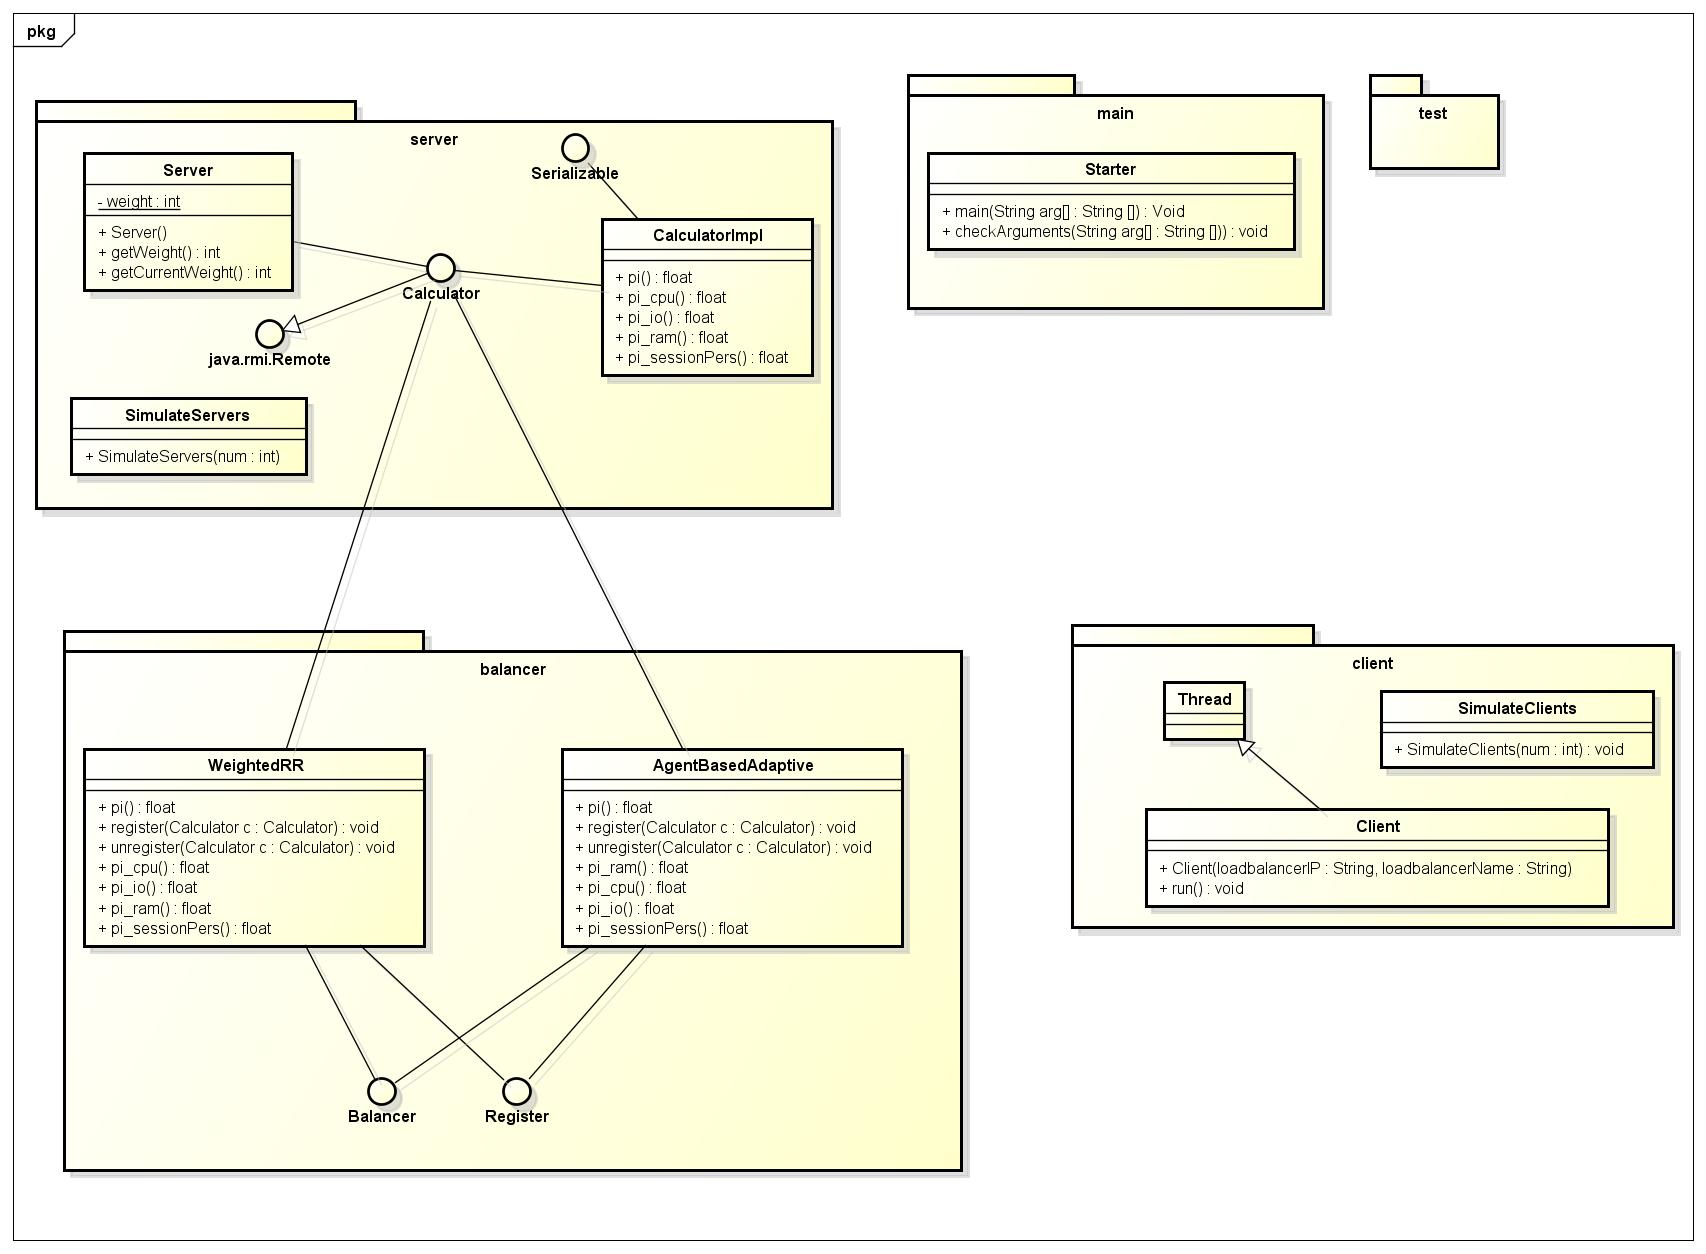
\includegraphics[width=1.0\textwidth]{images/cd1}
    \caption{Class Diagram First Try}
    \label{fig:cpu1}
\end{figure}
\begin{figure}[here!]
\centering
    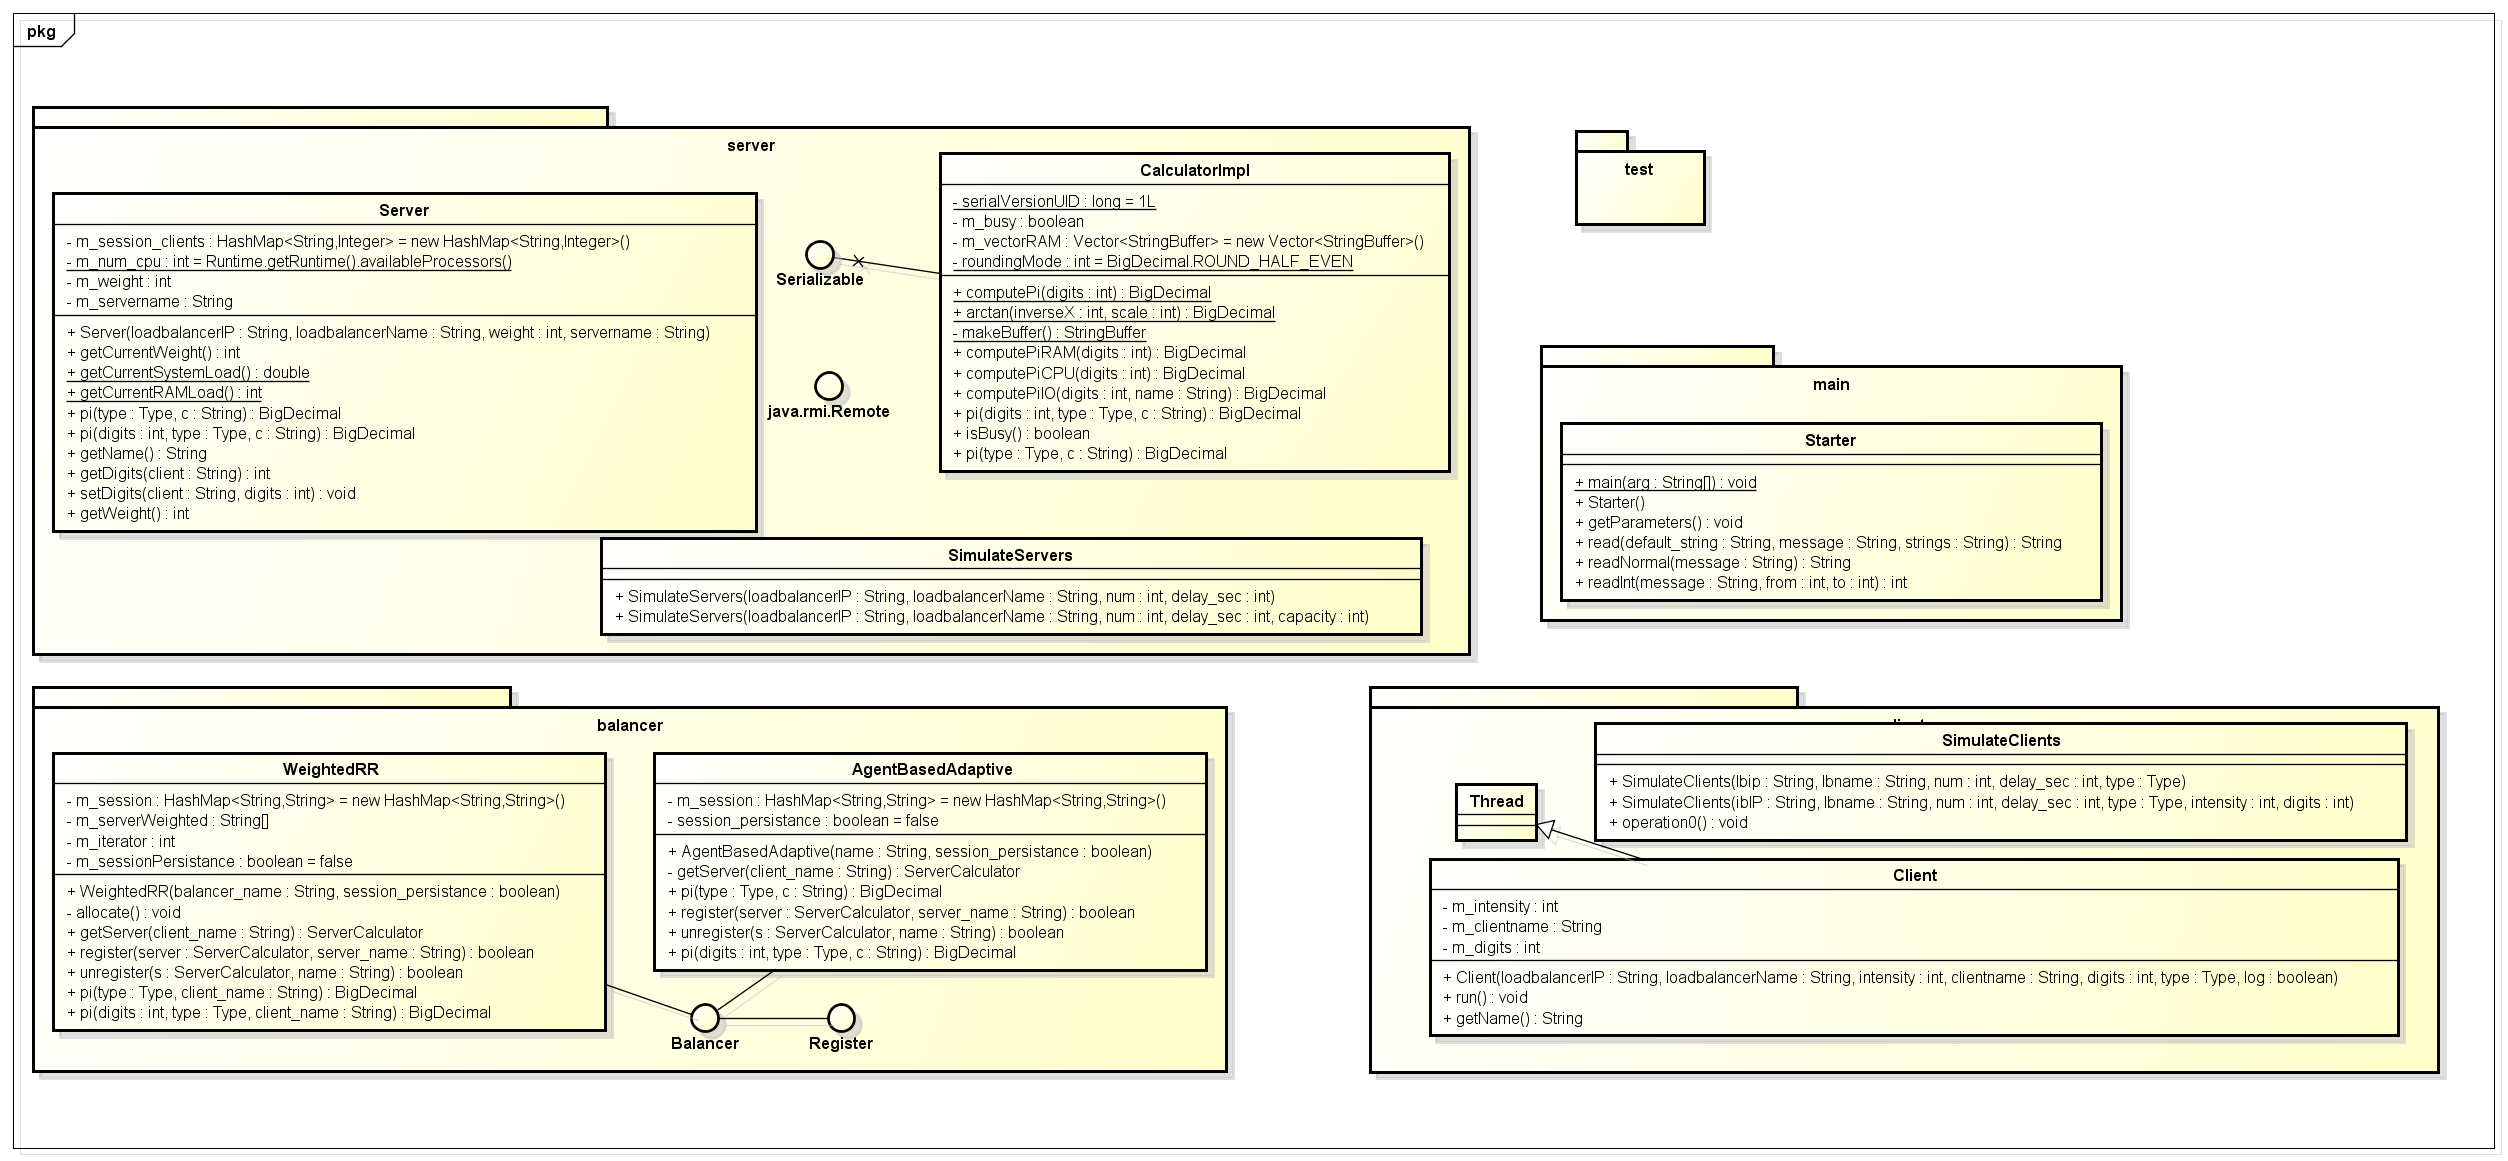
\includegraphics[width=1.0\textwidth]{images/cd2}
    \caption{Final Class Diagram}
    \label{fig:cpu1}
\end{figure}
\FloatBarrier
\subsection{Basic Load Balancing Scaffold} 
\subsubsection{Starter class}
We have done a \texttt{Starter} class, where the components were stared and a dialog for getting the informations from the user.
\subsubsection{Interfaces}
We have defined some Interfaces:
\begin{itemize}
\item Calculator
\item Server
\item Register
\item ServerCalculator (Calculator and Server interface)
\item Balancer (Register and Calculator interface)
\end{itemize}
\newpage
\subsubsection{Basic Load Balancer}
The Load Balancer uses RMI:
\begin{lstlisting}    
Balancer x;
// Exporting stub
try {
	x = (Balancer) UnicastRemoteObject.exportObject(this, 0);

	// creating the registry
	Registry registry = LocateRegistry.createRegistry(1099);

	// binding Balancer
	registry.bind(balancer_name, x);
} catch (AlreadyBoundException e) {
	Log.error("Load Balancer already bound, can not bound it again",e);
} catch (RemoteException e) {
	Log.error("There was a remote exception while exporting the Object",e);
}
\end{lstlisting}    
This is as usually, we basically have copied it from last year's task.
\subsubsection{Client}
The Client is a Thread. It has a specific number of digits which it demands from the server.
It also has a specific intensity with which the client demands the Services.\\
There are different Types of 
\subsubsection{Server}
\begin{lstlisting}  		
// calculator object
m_calc = new CalculatorImpl();
		
//fetch registry
Registry registry = LocateRegistry.getRegistry(loadbalancerIP,1099);
			
//fetch balancer
m_balancer = (Balancer) registry.lookup(loadbalancerName);
		
ServerCalculator x;
//bind server
x = (ServerCalculator) UnicastRemoteObject.exportObject(this, 0);
			
m_balancer.register(x, servername);
\end{lstlisting}  
\subsubsection{Pi-Calculation}
The Pi Calculation has been copied from last years task.
\subsection{Weighted Round Robin} 
The Weighted Round Robin Load Balancer has an allocation method:
\begin{lstlisting}  
//all the servers
HashMap<String, Integer> availiable_servers = new HashMap<String, Integer>();

//fetching the information from the servers: <Servername, Weigth>
for (Entry entry : m_servers.entrySet()) {
    ServerCalculator obj = (ServerCalculator) entry.getValue();
	availiable_servers.put(entry.getKey().toString(),obj.getWeight());
}

//calculate total weigth (Sum from all the Weights)
...
Log.logAlg("Allocation has found out a total amount of " + number + " units");

//generate servers array
String servers[] = new String[number];
int already_allocated = 0;
while (already_allocated < number) {
		...
}
//set the allocated values
  while (m_iterator != 0){}
  m_serverWeighted = servers;
\end{lstlisting}  
And he gets the next Server from the getServer method.
\begin{lstlisting}  
public ServerCalculator getServer(String client_name) throws RemoteException{
  if ( m_servers.size() <= 0){
	Log.logMax("There is no server which could handle this request!");
	return null;
  }
  else{
	//if session persistance should be used, 
	// and the client has already a server as a peer, 
	// and this server is still availiable...
		choosen_server = m_servers.get(m_session.get(client_name));		
		//if the server has to big of a load (90)
		if(!(choosen_server.getCurrentWeight()<90)){
			// choose different server	
		}
	
	//else 		
		//get the next server 'in line'
		choosen_server = (ServerCalculator) m_servers.get(server_weighted[m_iterator]);
		m_iterator++;
				
		//reset iterartor	
		if(m_iterator==server_weighted.length)
			m_iterator = 0;
	}		
  return choosen_server;
}
\end{lstlisting}  
\subsection{Agent Based Adaptive} 
The Agent Based Adaptive has only the getServer method which returns a Server.
\begin{lstlisting}  
if ( m_servers.size() <= 0){
  Log.logMax("There is no server which could handle this request!");
  return null;
}
else{
	//if session persistance should be used, 
	// and the client has already a server as a peer, 
	// and this server is still availiable...
		choosen_server = m_servers.get(m_session.get(client_name));		
		//if the server has to big of a load (90)
		if(!(choosen_server.getCurrentWeight()<90)){
			// choose different server	
		}
	//else
	  int smallest_load = 101;
 	  
 	  //find the server with the smallest load
	  for (Entry entry : m_servers.entrySet()) {
	     ...
	  }
				
	  // get the server object
	  choosen_server =  m_servers.get(servers_capacities);
				
	  return choosen_server;
\end{lstlisting}  

\subsection{Session Persistence}
We have implemented the session persistence. We thought, that in order to 'proof' that it works, we will simply let the client make 3 requests and see if it works and then let him make 1 request without any specifications of it's digits. \\
The server will then know (because the session persistance is implemented and therefore the client always gets the same server which stores the information) how many digits to give back to the client.
This is actually working. Only if the servers load is bigger than 90, the Client will get a new peer, but the information is going to be transferred.
\begin{figure}[here!]
\centering
    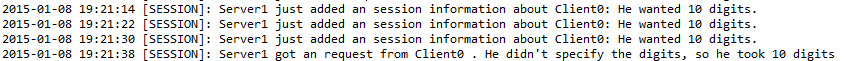
\includegraphics[width=1.0\textwidth]{images/sp}
    \caption{Session Persistence - digit information successfully retrieved}
    \label{fig:sp}
\end{figure}
\begin{figure}[here!]
\centering
    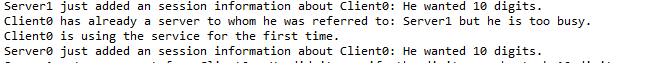
\includegraphics[width=1.0\textwidth]{images/sp2}
    \caption{Session Persistence - if the server was too busy}
    \label{fig:sp2}
\end{figure}
\subsection{Testing with CPU, RAM and I/O} 
We asked the User when starting what kind of type should be done.
Either the CPU will be used, a lot of RAM or an I/O should be implemented. \\
\subsubsection{CPU}
We simply did a useless Pi computing after returning the right value. That this works can be seen in Figure \ref{fig:cpu1}.
\begin{lstlisting}		
public BigDecimal computePiCPU(int digits) {
  //do some useless things
  computePi(digits*100000);
		
  return computePi(digits);
}
\end{lstlisting}
\begin{figure}[here!]
\centering
    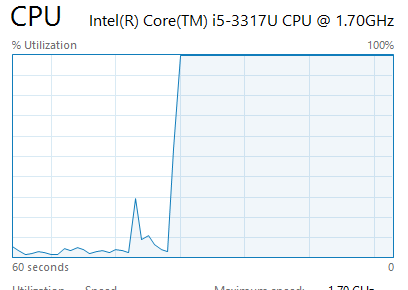
\includegraphics[width=0.5\textwidth]{images/cpu1}
    \caption{CPU usage}
    \label{fig:cpu1}
\end{figure}
\subsubsection{RAM}
The Ram was overfloated using a String Buffer: 
\begin{lstlisting}
public BigDecimal computePiRAM(int digits) {
  //adding stuff to RAM
  StringBuffer b = makeBuffer();
  m_vectorRAM.addElement(b);
  return computePi(digits);
}
\end{lstlisting}
\subsubsection{IO}
\begin{lstlisting}

public BigDecimal computePiIO(int digits,String name) {
		StringBuffer b = makeBuffer();
		FileOutputStream fo = null;
		PrintWriter pw = null;
		try {
			File f = new File("C:/temp/myfile"+name+".txt");
			f.deleteOnExit();
			fo = new FileOutputStream(f);
			pw = new PrintWriter(fo,true);
			pw.println(b.toString());
			pw.close();
			fo.close();
		} catch (FileNotFoundException e) {
			Log.error("Could not find File", e);
		} catch (IOException e) {
			Log.error("There occured a IO Exception...", e);
		}
		
		return computePi(digits);
}
\end{lstlisting}
\subsubsection{Implementing CPU, RAM and IO} 
\textbf{RAM}\\
The Ram was computed using the following code:
\begin{lstlisting}
public static int getCurrentRAMLoad(){
  int res = 0;
  Runtime runtime = Runtime.getRuntime();
  long ram_availiabe=runtime.totalMemory();
  long ram_used = runtime.totalMemory() - runtime.freeMemory();
		
  res  = (int)( ((100.0 / (double)ram_availiabe)*(double)ram_used)+0.5);
  return res;
}	
\end{lstlisting}
\textbf{CPU}\\
As it can be seen in the Problems section, the CPU with Java and Windows was not possible, at least not with normal APIs. We than decided not to implement this, because this took too long.
\section{Testing}
Testing has not be finished yet. Until now everything worked fine.
%\subsection{Screenshots}
%TODO
\subsection{JUnit}
We have not yet found the time to implement JUnit Test cases.
\section{Comparison between the Load Balancing Algorithms}
Both Algorithms work equally fine. \\
The Weighted Round Robin is hard to test, because we only do have two laptops.
For calculating the Current Weight, the CPU of the system is needed, but we were not able to retrieve it.
So we simulated it, which is not perfect either.
\\ \\
We think that the Weighted Round Robin Algorithm is great whenever the Connections are short and require only easy calculations. The Agent Based Adaptive Algorithm would be better if there were time consuming Requests, which request more difficult operations. \\
Other than that, we also have seen that the session persistence takes the scheduling away from the Balancer, because it kind of skips the algorithm if there is one server already assigned to a client.
\section{Problems}
\subsubsection{Log4j}
We were not able to include Log4j. There was a new version and we couldn't find a useful hint on the internet.
Therefore we simply wrote our own Log-class.
\subsubsection{RMI over Network didn't work}
The RMI Network communication was not working. \\
The bug was fixed when the Virtual machine networks were turned off. \\ \\
Mr. Borko then told us, that the interface was simply missing.
\subsubsection{Calculating the CPU Load}
We were not able to calculate the cpu load. The most promising answer was found under \cite{cpuload}, but this simply returned -1. \\
Other than that external libraries must be used.

\end{document}

\subsection{Easy Bibliography}
\begin{thebibliography}{56}
 http://mariemjabloun.blogspot.co.at/2014/09/log4j-2-tutorial-solve-error.html

 \bibitem{cpuload} 
  \textbf{CPU load from Java}, paweloque, Mar 11 '09 at 13:48\\
  \textit{  http://stackoverflow.com/questions/634580/cpu-load-from-java}
  \newline last used: 01.01.2014, 17:00
  
  
  \bibitem{example} 
  \textbf{Mister Super-genious}, Answer from 20.01.2015\\
  \textit{http://www.stackoverflow.com/question}
  \newline last used: 22.10.2014, 21:00

\end{thebibliography}
\end{document}
